\documentclass[1p]{elsarticle_modified}
%\bibliographystyle{elsarticle-num}

%\usepackage[colorlinks]{hyperref}
%\usepackage{abbrmath_seonhwa} %\Abb, \Ascr, \Acal ,\Abf, \Afrak
\usepackage{amsfonts}
\usepackage{amssymb}
\usepackage{amsmath}
\usepackage{amsthm}
\usepackage{scalefnt}
\usepackage{amsbsy}
\usepackage{kotex}
\usepackage{caption}
\usepackage{subfig}
\usepackage{color}
\usepackage{graphicx}
\usepackage{xcolor} %% white, black, red, green, blue, cyan, magenta, yellow
\usepackage{float}
\usepackage{setspace}
\usepackage{hyperref}

\usepackage{tikz}
\usetikzlibrary{arrows}

\usepackage{multirow}
\usepackage{array} % fixed length table
\usepackage{hhline}

%%%%%%%%%%%%%%%%%%%%%
\makeatletter
\renewcommand*\env@matrix[1][\arraystretch]{%
	\edef\arraystretch{#1}%
	\hskip -\arraycolsep
	\let\@ifnextchar\new@ifnextchar
	\array{*\c@MaxMatrixCols c}}
\makeatother %https://tex.stackexchange.com/questions/14071/how-can-i-increase-the-line-spacing-in-a-matrix
%%%%%%%%%%%%%%%

\usepackage[normalem]{ulem}

\newcommand{\msout}[1]{\ifmmode\text{\sout{\ensuremath{#1}}}\else\sout{#1}\fi}
%SOURCE: \msout is \stkout macro in https://tex.stackexchange.com/questions/20609/strikeout-in-math-mode

\newcommand{\cancel}[1]{
	\ifmmode
	{\color{red}\msout{#1}}
	\else
	{\color{red}\sout{#1}}
	\fi
}

\newcommand{\add}[1]{
	{\color{blue}\uwave{#1}}
}

\newcommand{\replace}[2]{
	\ifmmode
	{\color{red}\msout{#1}}{\color{blue}\uwave{#2}}
	\else
	{\color{red}\sout{#1}}{\color{blue}\uwave{#2}}
	\fi
}

\newcommand{\Sol}{\mathcal{S}} %segment
\newcommand{\D}{D} %diagram
\newcommand{\A}{\mathcal{A}} %arc


%%%%%%%%%%%%%%%%%%%%%%%%%%%%%5 test

\def\sl{\operatorname{\textup{SL}}(2,\Cbb)}
\def\psl{\operatorname{\textup{PSL}}(2,\Cbb)}
\def\quan{\mkern 1mu \triangleright \mkern 1mu}

\theoremstyle{definition}
\newtheorem{thm}{Theorem}[section]
\newtheorem{prop}[thm]{Proposition}
\newtheorem{lem}[thm]{Lemma}
\newtheorem{ques}[thm]{Question}
\newtheorem{cor}[thm]{Corollary}
\newtheorem{defn}[thm]{Definition}
\newtheorem{exam}[thm]{Example}
\newtheorem{rmk}[thm]{Remark}
\newtheorem{alg}[thm]{Algorithm}

\newcommand{\I}{\sqrt{-1}}
\begin{document}

%\begin{frontmatter}
%
%\title{Boundary parabolic representations of knots up to 8 crossings}
%
%%% Group authors per affiliation:
%\author{Yunhi Cho} 
%\address{Department of Mathematics, University of Seoul, Seoul, Korea}
%\ead{yhcho@uos.ac.kr}
%
%
%\author{Seonhwa Kim} %\fnref{s_kim}}
%\address{Center for Geometry and Physics, Institute for Basic Science, Pohang, 37673, Korea}
%\ead{ryeona17@ibs.re.kr}
%
%\author{Hyuk Kim}
%\address{Department of Mathematical Sciences, Seoul National University, Seoul 08826, Korea}
%\ead{hyukkim@snu.ac.kr}
%
%\author{Seokbeom Yoon}
%\address{Department of Mathematical Sciences, Seoul National University, Seoul, 08826,  Korea}
%\ead{sbyoon15@snu.ac.kr}
%
%\begin{abstract}
%We find all boundary parabolic representation of knots up to 8 crossings.
%
%\end{abstract}
%\begin{keyword}
%    \MSC[2010] 57M25 
%\end{keyword}
%
%\end{frontmatter}

%\linenumbers
%\tableofcontents
%
\newcommand\colored[1]{\textcolor{white}{\rule[-0.35ex]{0.8em}{1.4ex}}\kern-0.8em\color{red} #1}%
%\newcommand\colored[1]{\textcolor{white}{ #1}\kern-2.17ex	\textcolor{white}{ #1}\kern-1.81ex	\textcolor{white}{ #1}\kern-2.15ex\color{red}#1	}

{\Large $\underline{12a_{0077}~(K12a_{0077})}$}

\setlength{\tabcolsep}{10pt}
\renewcommand{\arraystretch}{1.6}
\vspace{1cm}\begin{tabular}{m{100pt}>{\centering\arraybackslash}m{274pt}}
\multirow{5}{120pt}{
	\centering
	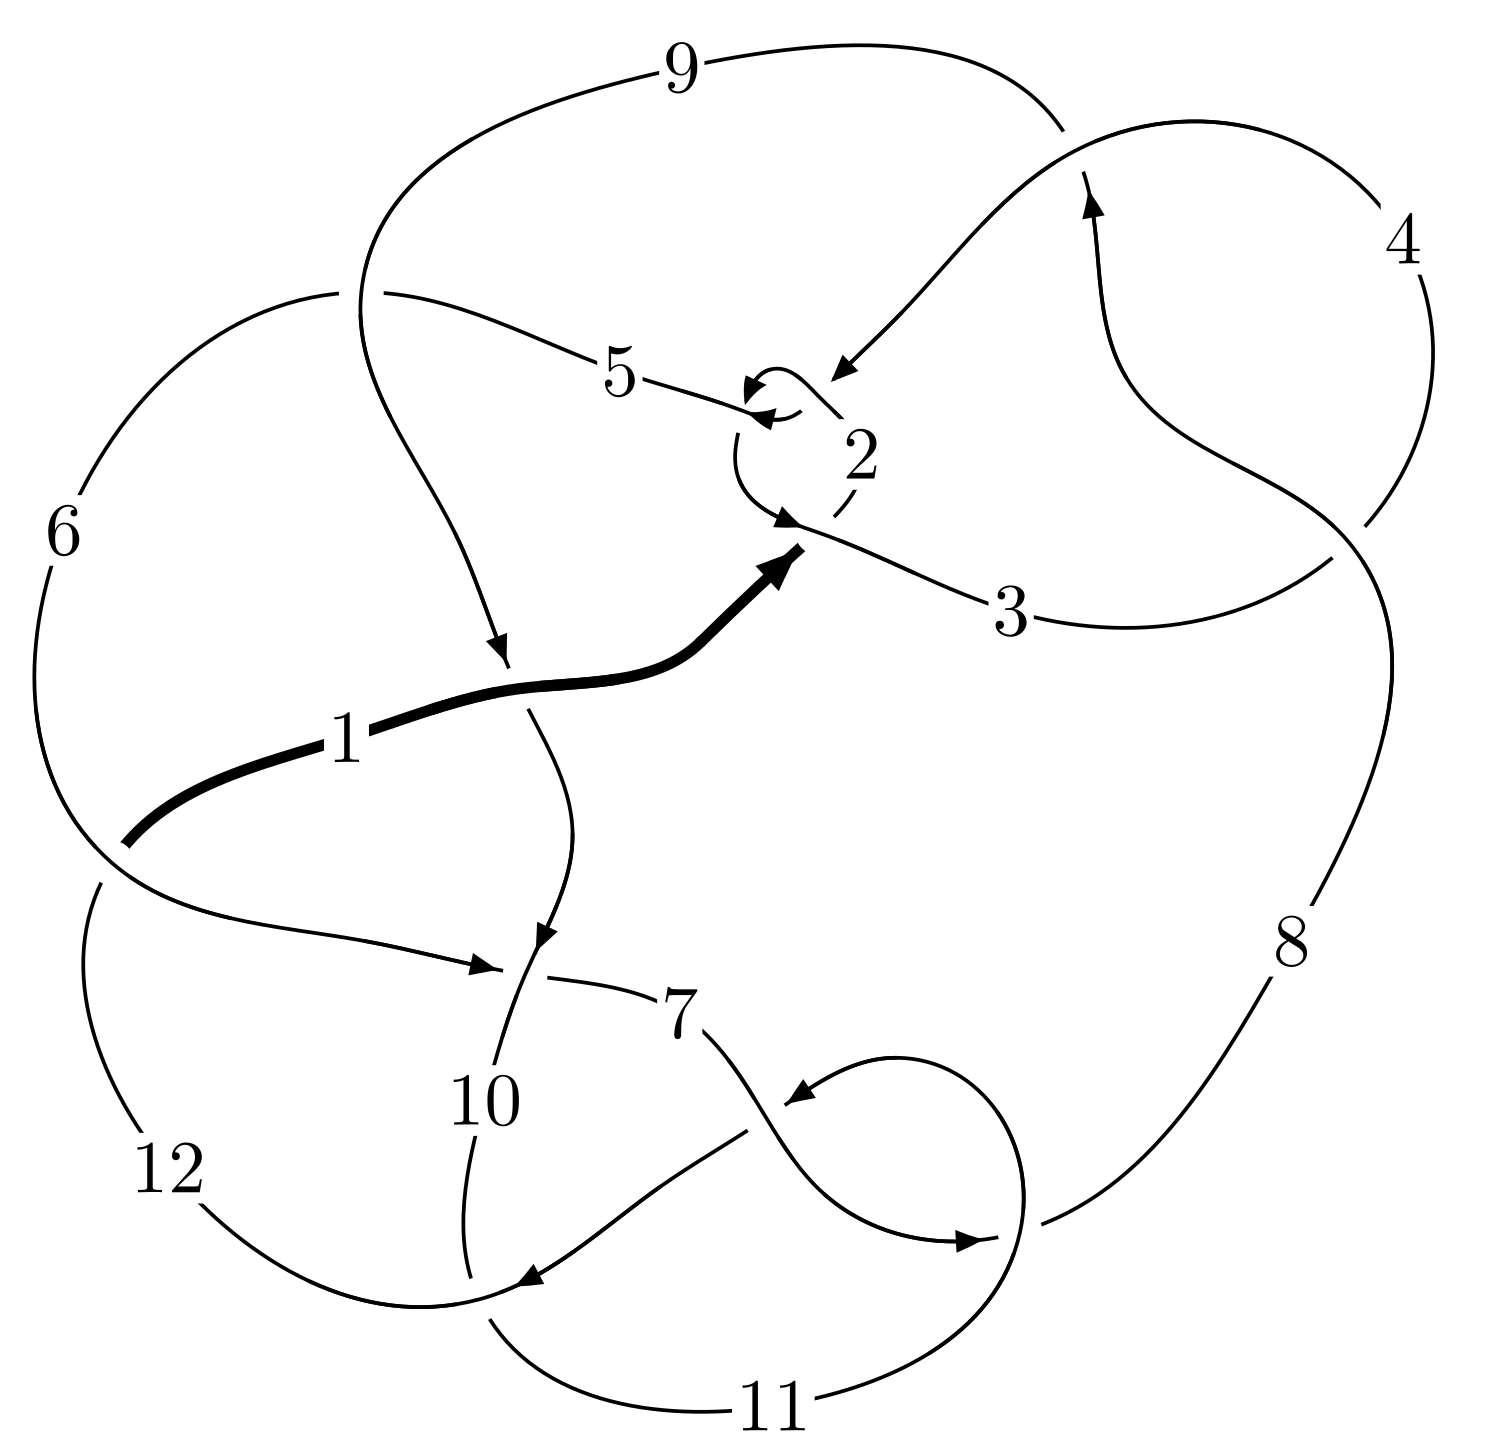
\includegraphics[width=112pt]{../../../GIT/diagram.site/Diagrams/png/878_12a_0077.png}\\
\ \ \ A knot diagram\footnotemark}&
\allowdisplaybreaks
\textbf{Linearized knot diagam} \\
\cline{2-2}
 &
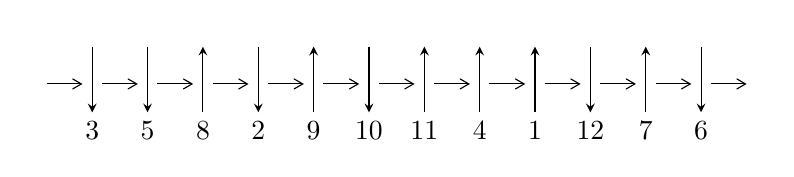
\begin{tikzpicture}[x=20pt, y=17pt]
	% nodes
	\node (C0) at (0, 0) {};
	\node (C1) at (1, 0) {};
	\node (C1U) at (1, +1) {};
	\node (C1D) at (1, -1) {3};

	\node (C2) at (2, 0) {};
	\node (C2U) at (2, +1) {};
	\node (C2D) at (2, -1) {5};

	\node (C3) at (3, 0) {};
	\node (C3U) at (3, +1) {};
	\node (C3D) at (3, -1) {8};

	\node (C4) at (4, 0) {};
	\node (C4U) at (4, +1) {};
	\node (C4D) at (4, -1) {2};

	\node (C5) at (5, 0) {};
	\node (C5U) at (5, +1) {};
	\node (C5D) at (5, -1) {9};

	\node (C6) at (6, 0) {};
	\node (C6U) at (6, +1) {};
	\node (C6D) at (6, -1) {10};

	\node (C7) at (7, 0) {};
	\node (C7U) at (7, +1) {};
	\node (C7D) at (7, -1) {11};

	\node (C8) at (8, 0) {};
	\node (C8U) at (8, +1) {};
	\node (C8D) at (8, -1) {4};

	\node (C9) at (9, 0) {};
	\node (C9U) at (9, +1) {};
	\node (C9D) at (9, -1) {1};

	\node (C10) at (10, 0) {};
	\node (C10U) at (10, +1) {};
	\node (C10D) at (10, -1) {12};

	\node (C11) at (11, 0) {};
	\node (C11U) at (11, +1) {};
	\node (C11D) at (11, -1) {7};

	\node (C12) at (12, 0) {};
	\node (C12U) at (12, +1) {};
	\node (C12D) at (12, -1) {6};
	\node (C13) at (13, 0) {};

	% arrows
	\draw[->,>={angle 60}]
	(C0) edge (C1) (C1) edge (C2) (C2) edge (C3) (C3) edge (C4) (C4) edge (C5) (C5) edge (C6) (C6) edge (C7) (C7) edge (C8) (C8) edge (C9) (C9) edge (C10) (C10) edge (C11) (C11) edge (C12) (C12) edge (C13) ;	\draw[->,>=stealth]
	(C1U) edge (C1D) (C2U) edge (C2D) (C3D) edge (C3U) (C4U) edge (C4D) (C5D) edge (C5U) (C6U) edge (C6D) (C7D) edge (C7U) (C8D) edge (C8U) (C9D) edge (C9U) (C10U) edge (C10D) (C11D) edge (C11U) (C12U) edge (C12D) ;
	\end{tikzpicture} \\
\hhline{~~} \\& 
\textbf{Solving Sequence} \\ \cline{2-2} 
 &
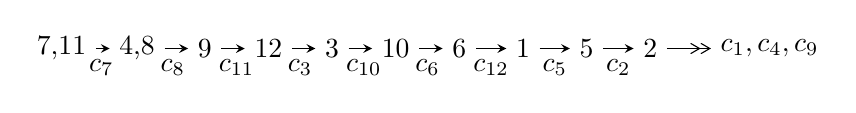
\begin{tikzpicture}[x=23pt, y=7pt]
	% node
	\node (A0) at (-1/8, 0) {7,11};
	\node (A1) at (17/16, 0) {4,8};
	\node (A2) at (17/8, 0) {9};
	\node (A3) at (25/8, 0) {12};
	\node (A4) at (33/8, 0) {3};
	\node (A5) at (41/8, 0) {10};
	\node (A6) at (49/8, 0) {6};
	\node (A7) at (57/8, 0) {1};
	\node (A8) at (65/8, 0) {5};
	\node (A9) at (73/8, 0) {2};
	\node (C1) at (1/2, -1) {$c_{7}$};
	\node (C2) at (13/8, -1) {$c_{8}$};
	\node (C3) at (21/8, -1) {$c_{11}$};
	\node (C4) at (29/8, -1) {$c_{3}$};
	\node (C5) at (37/8, -1) {$c_{10}$};
	\node (C6) at (45/8, -1) {$c_{6}$};
	\node (C7) at (53/8, -1) {$c_{12}$};
	\node (C8) at (61/8, -1) {$c_{5}$};
	\node (C9) at (69/8, -1) {$c_{2}$};
	\node (A10) at (11, 0) {$c_{1},c_{4},c_{9}$};

	% edge
	\draw[->,>=stealth]	
	(A0) edge (A1) (A1) edge (A2) (A2) edge (A3) (A3) edge (A4) (A4) edge (A5) (A5) edge (A6) (A6) edge (A7) (A7) edge (A8) (A8) edge (A9) ;
	\draw[->>,>={angle 60}]	
	(A9) edge (A10);
\end{tikzpicture} \\ 

\end{tabular} \\

\footnotetext{
The image of knot diagram is generated by the software ``\textbf{Draw programme}" developed by Andrew Bartholomew(\url{http://www.layer8.co.uk/maths/draw/index.htm\#Running-draw}), where we modified some parts for our purpose(\url{https://github.com/CATsTAILs/LinksPainter}).
}\phantom \\ \newline 
\centering \textbf{Ideals for irreducible components\footnotemark of $X_{\text{par}}$} 
 
\begin{align*}
I^u_{1}&=\langle 
u^{121}+u^{120}+\cdots+b+u,\;u^{121}+u^{120}+\cdots+a- u,\;u^{122}+2 u^{121}+\cdots+3 u+1\rangle \\
I^u_{2}&=\langle 
b- u,\;- u^3+a- u-1,\;u^4+u^2+u+1\rangle \\
I^u_{3}&=\langle 
u^5- u^4+2 u^3-2 u^2+b+2 u-1,\;- u^4- u^2+a,\;u^6- u^5+2 u^4-2 u^3+2 u^2-2 u+1\rangle \\
\\
\end{align*}
\raggedright * 3 irreducible components of $\dim_{\mathbb{C}}=0$, with total 132 representations.\\
\footnotetext{All coefficients of polynomials are rational numbers. But the coefficients are sometimes approximated in decimal forms when there is not enough margin.}
\newpage
\renewcommand{\arraystretch}{1}
\centering \section*{I. $I^u_{1}= \langle u^{121}+u^{120}+\cdots+b+u,\;u^{121}+u^{120}+\cdots+a- u,\;u^{122}+2 u^{121}+\cdots+3 u+1 \rangle$}
\flushleft \textbf{(i) Arc colorings}\\
\begin{tabular}{m{7pt} m{180pt} m{7pt} m{180pt} }
\flushright $a_{7}=$&$\begin{pmatrix}1\\0\end{pmatrix}$ \\
\flushright $a_{11}=$&$\begin{pmatrix}0\\u\end{pmatrix}$ \\
\flushright $a_{4}=$&$\begin{pmatrix}- u^{121}- u^{120}+\cdots-4 u^3+u\\- u^{121}- u^{120}+\cdots-3 u^2- u\end{pmatrix}$ \\
\flushright $a_{8}=$&$\begin{pmatrix}1\\- u^2\end{pmatrix}$ \\
\flushright $a_{9}=$&$\begin{pmatrix}u^{19}+4 u^{17}+8 u^{15}+8 u^{13}+3 u^{11}-2 u^9-2 u^7+u^3\\u^{19}+5 u^{17}+12 u^{15}+17 u^{13}+15 u^{11}+9 u^9+4 u^7+2 u^5+u^3+u\end{pmatrix}$ \\
\flushright $a_{12}=$&$\begin{pmatrix}u\\u\end{pmatrix}$ \\
\flushright $a_{3}=$&$\begin{pmatrix}u^{120}+u^{119}+\cdots+4 u+1\\u^{120}- u^{119}+\cdots-2 u^3- u^2\end{pmatrix}$ \\
\flushright $a_{10}=$&$\begin{pmatrix}u^3\\u^3+u\end{pmatrix}$ \\
\flushright $a_{6}=$&$\begin{pmatrix}- u^6- u^4+1\\- u^6-2 u^4- u^2\end{pmatrix}$ \\
\flushright $a_{1}=$&$\begin{pmatrix}u^{11}+2 u^9+2 u^7- u^3\\u^{11}+3 u^9+4 u^7+3 u^5+u^3+u\end{pmatrix}$ \\
\flushright $a_{5}=$&$\begin{pmatrix}u^{32}+7 u^{30}+\cdots+2 u^{12}+1\\u^{32}+8 u^{30}+\cdots+12 u^8+4 u^6\end{pmatrix}$ \\
\flushright $a_{2}=$&$\begin{pmatrix}u^{117}+u^{116}+\cdots+3 u+1\\- u^{119}- u^{118}+\cdots-3 u^3-2 u^2\end{pmatrix}$\\&\end{tabular}
\flushleft \textbf{(ii) Obstruction class $= -1$}\\~\\
\flushleft \textbf{(iii) Cusp Shapes $= 4 u^{121}+16 u^{120}+\cdots+25 u+10$}\\~\\
\newpage\renewcommand{\arraystretch}{1}
\flushleft \textbf{(iv) u-Polynomials at the component}\newline \\
\begin{tabular}{m{50pt}|m{274pt}}
Crossings & \hspace{64pt}u-Polynomials at each crossing \\
\hline $$\begin{aligned}c_{1}\end{aligned}$$&$\begin{aligned}
&u^{122}+57 u^{121}+\cdots-6 u+1
\end{aligned}$\\
\hline $$\begin{aligned}c_{2},c_{4}\end{aligned}$$&$\begin{aligned}
&u^{122}-11 u^{121}+\cdots-10 u+1
\end{aligned}$\\
\hline $$\begin{aligned}c_{3},c_{8}\end{aligned}$$&$\begin{aligned}
&u^{122}+u^{121}+\cdots+3072 u+1024
\end{aligned}$\\
\hline $$\begin{aligned}c_{5}\end{aligned}$$&$\begin{aligned}
&u^{122}-2 u^{121}+\cdots-8688533 u+4045417
\end{aligned}$\\
\hline $$\begin{aligned}c_{6}\end{aligned}$$&$\begin{aligned}
&u^{122}+2 u^{121}+\cdots+45832 u+4360
\end{aligned}$\\
\hline $$\begin{aligned}c_{7},c_{11}\end{aligned}$$&$\begin{aligned}
&u^{122}-2 u^{121}+\cdots-3 u+1
\end{aligned}$\\
\hline $$\begin{aligned}c_{9}\end{aligned}$$&$\begin{aligned}
&u^{122}+14 u^{121}+\cdots+8849 u+409
\end{aligned}$\\
\hline $$\begin{aligned}c_{10}\end{aligned}$$&$\begin{aligned}
&u^{122}+58 u^{121}+\cdots+5 u+1
\end{aligned}$\\
\hline $$\begin{aligned}c_{12}\end{aligned}$$&$\begin{aligned}
&u^{122}-10 u^{121}+\cdots-24512 u+5824
\end{aligned}$\\
\hline
\end{tabular}\\~\\
\newpage\renewcommand{\arraystretch}{1}
\flushleft \textbf{(v) Riley Polynomials at the component}\newline \\
\begin{tabular}{m{50pt}|m{274pt}}
Crossings & \hspace{64pt}Riley Polynomials at each crossing \\
\hline $$\begin{aligned}c_{1}\end{aligned}$$&$\begin{aligned}
&y^{122}+27 y^{121}+\cdots-66 y+1
\end{aligned}$\\
\hline $$\begin{aligned}c_{2},c_{4}\end{aligned}$$&$\begin{aligned}
&y^{122}-57 y^{121}+\cdots+6 y+1
\end{aligned}$\\
\hline $$\begin{aligned}c_{3},c_{8}\end{aligned}$$&$\begin{aligned}
&y^{122}-63 y^{121}+\cdots-30932992 y+1048576
\end{aligned}$\\
\hline $$\begin{aligned}c_{5}\end{aligned}$$&$\begin{aligned}
&y^{122}-38 y^{121}+\cdots-180991027544255 y+16365398703889
\end{aligned}$\\
\hline $$\begin{aligned}c_{6}\end{aligned}$$&$\begin{aligned}
&y^{122}-30 y^{121}+\cdots-1148670864 y+19009600
\end{aligned}$\\
\hline $$\begin{aligned}c_{7},c_{11}\end{aligned}$$&$\begin{aligned}
&y^{122}+58 y^{121}+\cdots+5 y+1
\end{aligned}$\\
\hline $$\begin{aligned}c_{9}\end{aligned}$$&$\begin{aligned}
&y^{122}+22 y^{121}+\cdots+25546025 y+167281
\end{aligned}$\\
\hline $$\begin{aligned}c_{10}\end{aligned}$$&$\begin{aligned}
&y^{122}+14 y^{121}+\cdots+13 y+1
\end{aligned}$\\
\hline $$\begin{aligned}c_{12}\end{aligned}$$&$\begin{aligned}
&y^{122}+26 y^{121}+\cdots+3082177920 y+33918976
\end{aligned}$\\
\hline
\end{tabular}\\~\\
\newpage\flushleft \textbf{(vi) Complex Volumes and Cusp Shapes}
$$\begin{array}{c|c|c}  
\text{Solutions to }I^u_{1}& \I (\text{vol} + \sqrt{-1}CS) & \text{Cusp shape}\\
 \hline 
\begin{aligned}
u &= -0.147503 + 1.019890 I \\
a &= \phantom{-}0.160638 + 0.361005 I \\
b &= \phantom{-}1.257490 - 0.009631 I\end{aligned}
 & \phantom{-}0.80605 - 4.42181 I & \phantom{-0.000000 } 0 \\ \hline\begin{aligned}
u &= -0.147503 - 1.019890 I \\
a &= \phantom{-}0.160638 - 0.361005 I \\
b &= \phantom{-}1.257490 + 0.009631 I\end{aligned}
 & \phantom{-}0.80605 + 4.42181 I & \phantom{-0.000000 } 0 \\ \hline\begin{aligned}
u &= -0.503910 + 0.793936 I \\
a &= \phantom{-}0.823657 + 0.701487 I \\
b &= \phantom{-}0.718290 + 0.623909 I\end{aligned}
 & \phantom{-}0.05395 - 4.08608 I & \phantom{-0.000000 } 0 \\ \hline\begin{aligned}
u &= -0.503910 - 0.793936 I \\
a &= \phantom{-}0.823657 - 0.701487 I \\
b &= \phantom{-}0.718290 - 0.623909 I\end{aligned}
 & \phantom{-}0.05395 + 4.08608 I & \phantom{-0.000000 } 0 \\ \hline\begin{aligned}
u &= -0.187037 + 1.064040 I \\
a &= -0.257633 + 0.087294 I \\
b &= -1.56569 + 0.12591 I\end{aligned}
 & \phantom{-}1.92349 + 0.97666 I & \phantom{-0.000000 } 0 \\ \hline\begin{aligned}
u &= -0.187037 - 1.064040 I \\
a &= -0.257633 - 0.087294 I \\
b &= -1.56569 - 0.12591 I\end{aligned}
 & \phantom{-}1.92349 - 0.97666 I & \phantom{-0.000000 } 0 \\ \hline\begin{aligned}
u &= \phantom{-}0.663437 + 0.631192 I \\
a &= -2.79895 + 0.94536 I \\
b &= -0.33616 + 1.66340 I\end{aligned}
 & \phantom{-}4.25458 + 10.76030 I & \phantom{-0.000000 } 0 \\ \hline\begin{aligned}
u &= \phantom{-}0.663437 - 0.631192 I \\
a &= -2.79895 - 0.94536 I \\
b &= -0.33616 - 1.66340 I\end{aligned}
 & \phantom{-}4.25458 - 10.76030 I & \phantom{-0.000000 } 0 \\ \hline\begin{aligned}
u &= \phantom{-}0.664047 + 0.613237 I \\
a &= \phantom{-}2.86898 - 0.94744 I \\
b &= \phantom{-}0.30798 - 1.84487 I\end{aligned}
 & \phantom{-}6.35315 + 5.04876 I & \phantom{-0.000000 } 0 \\ \hline\begin{aligned}
u &= \phantom{-}0.664047 - 0.613237 I \\
a &= \phantom{-}2.86898 + 0.94744 I \\
b &= \phantom{-}0.30798 + 1.84487 I\end{aligned}
 & \phantom{-}6.35315 - 5.04876 I & \phantom{-0.000000 } 0\\
 \hline 
 \end{array}$$\newpage$$\begin{array}{c|c|c}  
\text{Solutions to }I^u_{1}& \I (\text{vol} + \sqrt{-1}CS) & \text{Cusp shape}\\
 \hline 
\begin{aligned}
u &= \phantom{-}0.580897 + 0.939576 I \\
a &= \phantom{-}1.40599 - 0.64077 I \\
b &= \phantom{-}1.31558 - 2.50343 I\end{aligned}
 & \phantom{-}3.34514 - 5.92062 I & \phantom{-0.000000 } 0 \\ \hline\begin{aligned}
u &= \phantom{-}0.580897 - 0.939576 I \\
a &= \phantom{-}1.40599 + 0.64077 I \\
b &= \phantom{-}1.31558 + 2.50343 I\end{aligned}
 & \phantom{-}3.34514 + 5.92062 I & \phantom{-0.000000 } 0 \\ \hline\begin{aligned}
u &= -0.563945 + 0.687578 I \\
a &= -0.463939 - 0.933720 I \\
b &= -0.226560 - 0.728292 I\end{aligned}
 & \phantom{-}0.391182 - 0.219141 I & \phantom{-0.000000 } 0 \\ \hline\begin{aligned}
u &= -0.563945 - 0.687578 I \\
a &= -0.463939 + 0.933720 I \\
b &= -0.226560 + 0.728292 I\end{aligned}
 & \phantom{-}0.391182 + 0.219141 I & \phantom{-0.000000 } 0 \\ \hline\begin{aligned}
u &= \phantom{-}0.247747 + 1.082810 I \\
a &= \phantom{-}0.246194 + 1.053460 I \\
b &= \phantom{-}0.771686 + 0.150808 I\end{aligned}
 & -3.15692 + 0.14365 I & \phantom{-0.000000 } 0 \\ \hline\begin{aligned}
u &= \phantom{-}0.247747 - 1.082810 I \\
a &= \phantom{-}0.246194 - 1.053460 I \\
b &= \phantom{-}0.771686 - 0.150808 I\end{aligned}
 & -3.15692 - 0.14365 I & \phantom{-0.000000 } 0 \\ \hline\begin{aligned}
u &= -0.557353 + 0.961980 I \\
a &= \phantom{-}0.942594 - 0.238886 I \\
b &= \phantom{-}1.147840 - 0.156245 I\end{aligned}
 & \phantom{-}0.384580 - 0.022257 I & \phantom{-0.000000 } 0 \\ \hline\begin{aligned}
u &= -0.557353 - 0.961980 I \\
a &= \phantom{-}0.942594 + 0.238886 I \\
b &= \phantom{-}1.147840 + 0.156245 I\end{aligned}
 & \phantom{-}0.384580 + 0.022257 I & \phantom{-0.000000 } 0 \\ \hline\begin{aligned}
u &= -0.642511 + 0.606712 I \\
a &= \phantom{-}0.423802 - 1.223920 I \\
b &= \phantom{-}0.581380 - 0.647488 I\end{aligned}
 & \phantom{-}1.42902 - 4.68272 I & \phantom{-0.000000 } 0 \\ \hline\begin{aligned}
u &= -0.642511 - 0.606712 I \\
a &= \phantom{-}0.423802 + 1.223920 I \\
b &= \phantom{-}0.581380 + 0.647488 I\end{aligned}
 & \phantom{-}1.42902 + 4.68272 I & \phantom{-0.000000 } 0\\
 \hline 
 \end{array}$$\newpage$$\begin{array}{c|c|c}  
\text{Solutions to }I^u_{1}& \I (\text{vol} + \sqrt{-1}CS) & \text{Cusp shape}\\
 \hline 
\begin{aligned}
u &= \phantom{-}0.578496 + 0.957006 I \\
a &= -1.73350 + 0.73489 I \\
b &= -1.46493 + 2.74505 I\end{aligned}
 & \phantom{-}5.33977 - 0.21651 I & \phantom{-0.000000 } 0 \\ \hline\begin{aligned}
u &= \phantom{-}0.578496 - 0.957006 I \\
a &= -1.73350 - 0.73489 I \\
b &= -1.46493 - 2.74505 I\end{aligned}
 & \phantom{-}5.33977 + 0.21651 I & \phantom{-0.000000 } 0 \\ \hline\begin{aligned}
u &= \phantom{-}0.545074 + 0.978382 I \\
a &= \phantom{-}2.55909 - 0.38765 I \\
b &= \phantom{-}2.14304 - 3.11468 I\end{aligned}
 & -0.83283 + 2.32108 I & \phantom{-0.000000 } 0 \\ \hline\begin{aligned}
u &= \phantom{-}0.545074 - 0.978382 I \\
a &= \phantom{-}2.55909 + 0.38765 I \\
b &= \phantom{-}2.14304 + 3.11468 I\end{aligned}
 & -0.83283 - 2.32108 I & \phantom{-0.000000 } 0 \\ \hline\begin{aligned}
u &= \phantom{-}0.676980 + 0.556127 I \\
a &= \phantom{-}2.75159 - 0.80208 I \\
b &= \phantom{-}0.29221 - 2.16620 I\end{aligned}
 & \phantom{-}7.33859 + 0.89759 I & \phantom{-0.000000 } 0 \\ \hline\begin{aligned}
u &= \phantom{-}0.676980 - 0.556127 I \\
a &= \phantom{-}2.75159 + 0.80208 I \\
b &= \phantom{-}0.29221 + 2.16620 I\end{aligned}
 & \phantom{-}7.33859 - 0.89759 I & \phantom{-0.000000 } 0 \\ \hline\begin{aligned}
u &= \phantom{-}0.310246 + 1.083390 I \\
a &= -0.358349 + 1.021320 I \\
b &= \phantom{-}0.570849 + 0.641805 I\end{aligned}
 & -3.70234 + 0.56339 I & \phantom{-0.000000 } 0 \\ \hline\begin{aligned}
u &= \phantom{-}0.310246 - 1.083390 I \\
a &= -0.358349 - 1.021320 I \\
b &= \phantom{-}0.570849 - 0.641805 I\end{aligned}
 & -3.70234 - 0.56339 I & \phantom{-0.000000 } 0 \\ \hline\begin{aligned}
u &= \phantom{-}0.685820 + 0.531680 I \\
a &= -2.55763 + 0.78007 I \\
b &= -0.22955 + 2.19623 I\end{aligned}
 & \phantom{-}5.98830 - 4.81101 I & \phantom{-0.000000 } 0 \\ \hline\begin{aligned}
u &= \phantom{-}0.685820 - 0.531680 I \\
a &= -2.55763 - 0.78007 I \\
b &= -0.22955 - 2.19623 I\end{aligned}
 & \phantom{-}5.98830 + 4.81101 I & \phantom{-0.000000 } 0\\
 \hline 
 \end{array}$$\newpage$$\begin{array}{c|c|c}  
\text{Solutions to }I^u_{1}& \I (\text{vol} + \sqrt{-1}CS) & \text{Cusp shape}\\
 \hline 
\begin{aligned}
u &= -0.243131 + 1.108750 I \\
a &= \phantom{-}1.01081 - 1.20474 I \\
b &= \phantom{-}2.71881 - 0.53821 I\end{aligned}
 & -5.30960 + 1.62774 I & \phantom{-0.000000 } 0 \\ \hline\begin{aligned}
u &= -0.243131 - 1.108750 I \\
a &= \phantom{-}1.01081 + 1.20474 I \\
b &= \phantom{-}2.71881 + 0.53821 I\end{aligned}
 & -5.30960 - 1.62774 I & \phantom{-0.000000 } 0 \\ \hline\begin{aligned}
u &= -0.480136 + 1.029710 I \\
a &= \phantom{-}0.060217 + 0.435203 I \\
b &= \phantom{-}0.183899 + 0.551516 I\end{aligned}
 & -0.61714 - 3.08115 I & \phantom{-0.000000 } 0 \\ \hline\begin{aligned}
u &= -0.480136 - 1.029710 I \\
a &= \phantom{-}0.060217 - 0.435203 I \\
b &= \phantom{-}0.183899 - 0.551516 I\end{aligned}
 & -0.61714 + 3.08115 I & \phantom{-0.000000 } 0 \\ \hline\begin{aligned}
u &= \phantom{-}0.626554 + 0.591288 I \\
a &= -3.17061 + 0.97693 I \\
b &= -0.01997 + 2.10665 I\end{aligned}
 & \phantom{-}0.30602 + 2.29616 I & \phantom{-0.000000 } 0 \\ \hline\begin{aligned}
u &= \phantom{-}0.626554 - 0.591288 I \\
a &= -3.17061 - 0.97693 I \\
b &= -0.01997 - 2.10665 I\end{aligned}
 & \phantom{-}0.30602 - 2.29616 I & \phantom{-0.000000 } 0 \\ \hline\begin{aligned}
u &= \phantom{-}0.232311 + 1.117320 I \\
a &= -0.580972 - 1.076570 I \\
b &= -0.823114 + 0.039156 I\end{aligned}
 & -4.37882 - 4.12065 I & \phantom{-0.000000 } 0 \\ \hline\begin{aligned}
u &= \phantom{-}0.232311 - 1.117320 I \\
a &= -0.580972 + 1.076570 I \\
b &= -0.823114 - 0.039156 I\end{aligned}
 & -4.37882 + 4.12065 I & \phantom{-0.000000 } 0 \\ \hline\begin{aligned}
u &= -0.557153 + 0.997293 I \\
a &= -0.679241 + 0.573310 I \\
b &= -0.974590 + 0.622642 I\end{aligned}
 & \phantom{-}0.84323 - 4.34495 I & \phantom{-0.000000 } 0 \\ \hline\begin{aligned}
u &= -0.557153 - 0.997293 I \\
a &= -0.679241 - 0.573310 I \\
b &= -0.974590 - 0.622642 I\end{aligned}
 & \phantom{-}0.84323 + 4.34495 I & \phantom{-0.000000 } 0\\
 \hline 
 \end{array}$$\newpage$$\begin{array}{c|c|c}  
\text{Solutions to }I^u_{1}& \I (\text{vol} + \sqrt{-1}CS) & \text{Cusp shape}\\
 \hline 
\begin{aligned}
u &= -0.217849 + 1.124370 I \\
a &= -0.187626 + 1.188830 I \\
b &= -2.03552 + 0.87762 I\end{aligned}
 & \phantom{-}0.39410 + 4.66441 I & \phantom{-0.000000 } 0 \\ \hline\begin{aligned}
u &= -0.217849 - 1.124370 I \\
a &= -0.187626 - 1.188830 I \\
b &= -2.03552 - 0.87762 I\end{aligned}
 & \phantom{-}0.39410 - 4.66441 I & \phantom{-0.000000 } 0 \\ \hline\begin{aligned}
u &= -0.638088 + 0.561092 I \\
a &= -0.798780 + 0.964384 I \\
b &= -0.691669 + 0.304217 I\end{aligned}
 & \phantom{-}2.12882 - 0.34486 I & \phantom{-0.000000 } 0 \\ \hline\begin{aligned}
u &= -0.638088 - 0.561092 I \\
a &= -0.798780 - 0.964384 I \\
b &= -0.691669 - 0.304217 I\end{aligned}
 & \phantom{-}2.12882 + 0.34486 I & \phantom{-0.000000 } 0 \\ \hline\begin{aligned}
u &= -0.334748 + 1.103830 I \\
a &= -0.83313 - 1.90432 I \\
b &= -0.29049 - 2.26529 I\end{aligned}
 & -6.22983 - 1.88137 I & \phantom{-0.000000 } 0 \\ \hline\begin{aligned}
u &= -0.334748 - 1.103830 I \\
a &= -0.83313 + 1.90432 I \\
b &= -0.29049 + 2.26529 I\end{aligned}
 & -6.22983 + 1.88137 I & \phantom{-0.000000 } 0 \\ \hline\begin{aligned}
u &= -0.773736 + 0.340441 I \\
a &= -2.27642 + 0.95926 I \\
b &= -0.64290 - 2.33332 I\end{aligned}
 & \phantom{-}2.78144 + 13.02340 I & \phantom{-0.000000 } 0 \\ \hline\begin{aligned}
u &= -0.773736 - 0.340441 I \\
a &= -2.27642 - 0.95926 I \\
b &= -0.64290 + 2.33332 I\end{aligned}
 & \phantom{-}2.78144 - 13.02340 I & \phantom{-0.000000 } 0 \\ \hline\begin{aligned}
u &= -0.766387 + 0.349666 I \\
a &= \phantom{-}2.38500 - 0.93938 I \\
b &= \phantom{-}0.65193 + 2.19129 I\end{aligned}
 & \phantom{-}5.02651 + 7.30828 I & \phantom{-0.000000 } 0 \\ \hline\begin{aligned}
u &= -0.766387 - 0.349666 I \\
a &= \phantom{-}2.38500 + 0.93938 I \\
b &= \phantom{-}0.65193 - 2.19129 I\end{aligned}
 & \phantom{-}5.02651 - 7.30828 I & \phantom{-0.000000 } 0\\
 \hline 
 \end{array}$$\newpage$$\begin{array}{c|c|c}  
\text{Solutions to }I^u_{1}& \I (\text{vol} + \sqrt{-1}CS) & \text{Cusp shape}\\
 \hline 
\begin{aligned}
u &= \phantom{-}0.580775 + 1.002240 I \\
a &= -2.32556 + 1.16823 I \\
b &= -1.49852 + 3.23792 I\end{aligned}
 & \phantom{-}6.02309 + 3.97372 I & \phantom{-0.000000 } 0 \\ \hline\begin{aligned}
u &= \phantom{-}0.580775 - 1.002240 I \\
a &= -2.32556 - 1.16823 I \\
b &= -1.49852 - 3.23792 I\end{aligned}
 & \phantom{-}6.02309 - 3.97372 I & \phantom{-0.000000 } 0 \\ \hline\begin{aligned}
u &= -0.222634 + 1.137130 I \\
a &= \phantom{-}0.04620 - 1.47787 I \\
b &= \phantom{-}2.02261 - 1.14560 I\end{aligned}
 & -1.87191 + 10.28300 I & \phantom{-0.000000 } 0 \\ \hline\begin{aligned}
u &= -0.222634 - 1.137130 I \\
a &= \phantom{-}0.04620 + 1.47787 I \\
b &= \phantom{-}2.02261 + 1.14560 I\end{aligned}
 & -1.87191 - 10.28300 I & \phantom{-0.000000 } 0 \\ \hline\begin{aligned}
u &= -0.742446 + 0.388031 I \\
a &= \phantom{-}2.41605 - 0.76410 I \\
b &= \phantom{-}0.78560 + 1.54744 I\end{aligned}
 & \phantom{-}6.50957 + 3.19238 I & \phantom{-0.000000 } 0 \\ \hline\begin{aligned}
u &= -0.742446 - 0.388031 I \\
a &= \phantom{-}2.41605 + 0.76410 I \\
b &= \phantom{-}0.78560 - 1.54744 I\end{aligned}
 & \phantom{-}6.50957 - 3.19238 I & \phantom{-0.000000 } 0 \\ \hline\begin{aligned}
u &= -0.730426 + 0.409385 I \\
a &= -2.28243 + 0.74960 I \\
b &= -0.89107 - 1.21865 I\end{aligned}
 & \phantom{-}5.39473 - 2.49625 I & \phantom{-0.000000 } 0 \\ \hline\begin{aligned}
u &= -0.730426 - 0.409385 I \\
a &= -2.28243 - 0.74960 I \\
b &= -0.89107 + 1.21865 I\end{aligned}
 & \phantom{-}5.39473 + 2.49625 I & \phantom{-0.000000 } 0 \\ \hline\begin{aligned}
u &= \phantom{-}0.351696 + 1.109570 I \\
a &= \phantom{-}0.94996 - 1.25525 I \\
b &= -0.412184 - 1.221590 I\end{aligned}
 & -5.61386 + 4.27204 I & \phantom{-0.000000 } 0 \\ \hline\begin{aligned}
u &= \phantom{-}0.351696 - 1.109570 I \\
a &= \phantom{-}0.94996 + 1.25525 I \\
b &= -0.412184 + 1.221590 I\end{aligned}
 & -5.61386 - 4.27204 I & \phantom{-0.000000 } 0\\
 \hline 
 \end{array}$$\newpage$$\begin{array}{c|c|c}  
\text{Solutions to }I^u_{1}& \I (\text{vol} + \sqrt{-1}CS) & \text{Cusp shape}\\
 \hline 
\begin{aligned}
u &= \phantom{-}0.274646 + 1.138280 I \\
a &= -0.900239 - 0.382822 I \\
b &= -0.554801 + 0.399175 I\end{aligned}
 & -5.66097 + 1.23463 I & \phantom{-0.000000 } 0 \\ \hline\begin{aligned}
u &= \phantom{-}0.274646 - 1.138280 I \\
a &= -0.900239 + 0.382822 I \\
b &= -0.554801 - 0.399175 I\end{aligned}
 & -5.66097 - 1.23463 I & \phantom{-0.000000 } 0 \\ \hline\begin{aligned}
u &= \phantom{-}0.754006 + 0.343369 I \\
a &= \phantom{-}0.403285 - 0.833170 I \\
b &= -1.019380 - 0.886124 I\end{aligned}
 & \phantom{-}0.13714 - 6.77256 I & \phantom{-0.000000 -}0. + 5.74192 I \\ \hline\begin{aligned}
u &= \phantom{-}0.754006 - 0.343369 I \\
a &= \phantom{-}0.403285 + 0.833170 I \\
b &= -1.019380 + 0.886124 I\end{aligned}
 & \phantom{-}0.13714 + 6.77256 I & \phantom{-0.000000 } 0. - 5.74192 I \\ \hline\begin{aligned}
u &= \phantom{-}0.582684 + 1.018360 I \\
a &= \phantom{-}2.41797 - 1.26623 I \\
b &= \phantom{-}1.46594 - 3.24790 I\end{aligned}
 & \phantom{-}4.55439 + 9.71101 I & \phantom{-0.000000 } 0 \\ \hline\begin{aligned}
u &= \phantom{-}0.582684 - 1.018360 I \\
a &= \phantom{-}2.41797 + 1.26623 I \\
b &= \phantom{-}1.46594 + 3.24790 I\end{aligned}
 & \phantom{-}4.55439 - 9.71101 I & \phantom{-0.000000 } 0 \\ \hline\begin{aligned}
u &= -0.374798 + 1.116820 I \\
a &= \phantom{-}0.04976 + 1.74262 I \\
b &= -0.30164 + 1.53458 I\end{aligned}
 & -1.26418 - 4.75234 I & \phantom{-0.000000 } 0 \\ \hline\begin{aligned}
u &= -0.374798 - 1.116820 I \\
a &= \phantom{-}0.04976 - 1.74262 I \\
b &= -0.30164 - 1.53458 I\end{aligned}
 & -1.26418 + 4.75234 I & \phantom{-0.000000 } 0 \\ \hline\begin{aligned}
u &= \phantom{-}0.308936 + 1.138480 I \\
a &= \phantom{-}1.112100 - 0.379507 I \\
b &= \phantom{-}0.224418 - 0.838709 I\end{aligned}
 & -6.04051 - 1.73738 I & \phantom{-0.000000 } 0 \\ \hline\begin{aligned}
u &= \phantom{-}0.308936 - 1.138480 I \\
a &= \phantom{-}1.112100 + 0.379507 I \\
b &= \phantom{-}0.224418 + 0.838709 I\end{aligned}
 & -6.04051 + 1.73738 I & \phantom{-0.000000 } 0\\
 \hline 
 \end{array}$$\newpage$$\begin{array}{c|c|c}  
\text{Solutions to }I^u_{1}& \I (\text{vol} + \sqrt{-1}CS) & \text{Cusp shape}\\
 \hline 
\begin{aligned}
u &= -0.741592 + 0.341947 I \\
a &= -2.68131 + 1.04936 I \\
b &= -0.29140 - 2.09408 I\end{aligned}
 & -0.89417 + 4.25803 I & \phantom{-}2.47020 - 4.79794 I \\ \hline\begin{aligned}
u &= -0.741592 - 0.341947 I \\
a &= -2.68131 - 1.04936 I \\
b &= -0.29140 + 2.09408 I\end{aligned}
 & -0.89417 - 4.25803 I & \phantom{-}2.47020 + 4.79794 I \\ \hline\begin{aligned}
u &= \phantom{-}0.727560 + 0.357150 I \\
a &= -0.676826 + 0.613682 I \\
b &= \phantom{-}0.610983 + 1.066460 I\end{aligned}
 & \phantom{-}1.16636 - 2.32617 I & \phantom{-}3.33942 + 0. I\phantom{ +0.000000I} \\ \hline\begin{aligned}
u &= \phantom{-}0.727560 - 0.357150 I \\
a &= -0.676826 - 0.613682 I \\
b &= \phantom{-}0.610983 - 1.066460 I\end{aligned}
 & \phantom{-}1.16636 + 2.32617 I & \phantom{-}3.33942 + 0. I\phantom{ +0.000000I} \\ \hline\begin{aligned}
u &= -0.366393 + 1.135130 I \\
a &= \phantom{-}0.03793 - 2.08248 I \\
b &= \phantom{-}0.62048 - 1.73701 I\end{aligned}
 & -3.47259 - 10.00020 I & \phantom{-0.000000 } 0 \\ \hline\begin{aligned}
u &= -0.366393 - 1.135130 I \\
a &= \phantom{-}0.03793 + 2.08248 I \\
b &= \phantom{-}0.62048 + 1.73701 I\end{aligned}
 & -3.47259 + 10.00020 I & \phantom{-0.000000 } 0 \\ \hline\begin{aligned}
u &= -0.474706 + 1.099400 I \\
a &= -0.380284 + 0.418935 I \\
b &= \phantom{-}0.184497 + 0.371876 I\end{aligned}
 & -0.60185 - 2.76992 I & \phantom{-0.000000 } 0 \\ \hline\begin{aligned}
u &= -0.474706 - 1.099400 I \\
a &= -0.380284 - 0.418935 I \\
b &= \phantom{-}0.184497 - 0.371876 I\end{aligned}
 & -0.60185 + 2.76992 I & \phantom{-0.000000 } 0 \\ \hline\begin{aligned}
u &= \phantom{-}0.742897 + 0.291124 I \\
a &= -0.116461 - 0.570194 I \\
b &= -0.970990 + 0.058027 I\end{aligned}
 & -1.35964 - 1.73759 I & \phantom{-}2.29144 - 2.31325 I \\ \hline\begin{aligned}
u &= \phantom{-}0.742897 - 0.291124 I \\
a &= -0.116461 + 0.570194 I \\
b &= -0.970990 - 0.058027 I\end{aligned}
 & -1.35964 + 1.73759 I & \phantom{-}2.29144 + 2.31325 I\\
 \hline 
 \end{array}$$\newpage$$\begin{array}{c|c|c}  
\text{Solutions to }I^u_{1}& \I (\text{vol} + \sqrt{-1}CS) & \text{Cusp shape}\\
 \hline 
\begin{aligned}
u &= \phantom{-}0.505779 + 1.104550 I \\
a &= -1.00118 + 1.86287 I \\
b &= \phantom{-}0.58455 + 2.08301 I\end{aligned}
 & -4.58051 + 3.20726 I & \phantom{-0.000000 } 0 \\ \hline\begin{aligned}
u &= \phantom{-}0.505779 - 1.104550 I \\
a &= -1.00118 - 1.86287 I \\
b &= \phantom{-}0.58455 - 2.08301 I\end{aligned}
 & -4.58051 - 3.20726 I & \phantom{-0.000000 } 0 \\ \hline\begin{aligned}
u &= -0.519041 + 1.107540 I \\
a &= -0.142012 + 0.389842 I \\
b &= -1.316650 - 0.337487 I\end{aligned}
 & -4.97820 - 5.58195 I & \phantom{-0.000000 } 0 \\ \hline\begin{aligned}
u &= -0.519041 - 1.107540 I \\
a &= -0.142012 - 0.389842 I \\
b &= -1.316650 + 0.337487 I\end{aligned}
 & -4.97820 + 5.58195 I & \phantom{-0.000000 } 0 \\ \hline\begin{aligned}
u &= -0.484369 + 1.125250 I \\
a &= \phantom{-}0.819496 - 0.149267 I \\
b &= -0.112185 + 0.136501 I\end{aligned}
 & -2.68020 + 2.19171 I & \phantom{-0.000000 } 0 \\ \hline\begin{aligned}
u &= -0.484369 - 1.125250 I \\
a &= \phantom{-}0.819496 + 0.149267 I \\
b &= -0.112185 - 0.136501 I\end{aligned}
 & -2.68020 - 2.19171 I & \phantom{-0.000000 } 0 \\ \hline\begin{aligned}
u &= \phantom{-}0.536230 + 1.104700 I \\
a &= \phantom{-}1.03791 - 1.12148 I \\
b &= \phantom{-}0.04903 - 1.60825 I\end{aligned}
 & -2.15124 + 6.76591 I & \phantom{-0.000000 } 0 \\ \hline\begin{aligned}
u &= \phantom{-}0.536230 - 1.104700 I \\
a &= \phantom{-}1.03791 + 1.12148 I \\
b &= \phantom{-}0.04903 + 1.60825 I\end{aligned}
 & -2.15124 - 6.76591 I & \phantom{-0.000000 } 0 \\ \hline\begin{aligned}
u &= -0.576567 + 1.090460 I \\
a &= \phantom{-}0.82502 + 1.79493 I \\
b &= -0.26431 + 2.97096 I\end{aligned}
 & \phantom{-}3.39134 - 2.48781 I & \phantom{-0.000000 } 0 \\ \hline\begin{aligned}
u &= -0.576567 - 1.090460 I \\
a &= \phantom{-}0.82502 - 1.79493 I \\
b &= -0.26431 - 2.97096 I\end{aligned}
 & \phantom{-}3.39134 + 2.48781 I & \phantom{-0.000000 } 0\\
 \hline 
 \end{array}$$\newpage$$\begin{array}{c|c|c}  
\text{Solutions to }I^u_{1}& \I (\text{vol} + \sqrt{-1}CS) & \text{Cusp shape}\\
 \hline 
\begin{aligned}
u &= \phantom{-}0.715919 + 0.244608 I \\
a &= \phantom{-}0.402000 + 0.499492 I \\
b &= \phantom{-}0.881830 - 0.783285 I\end{aligned}
 & -1.99977 - 4.88959 I & -0.19185 + 6.83299 I \\ \hline\begin{aligned}
u &= \phantom{-}0.715919 - 0.244608 I \\
a &= \phantom{-}0.402000 - 0.499492 I \\
b &= \phantom{-}0.881830 + 0.783285 I\end{aligned}
 & -1.99977 + 4.88959 I & -0.19185 - 6.83299 I \\ \hline\begin{aligned}
u &= -0.576427 + 1.102190 I \\
a &= -1.22366 - 2.00645 I \\
b &= \phantom{-}0.14513 - 3.45387 I\end{aligned}
 & \phantom{-}4.40913 - 8.20349 I & \phantom{-0.000000 } 0 \\ \hline\begin{aligned}
u &= -0.576427 - 1.102190 I \\
a &= -1.22366 + 2.00645 I \\
b &= \phantom{-}0.14513 + 3.45387 I\end{aligned}
 & \phantom{-}4.40913 + 8.20349 I & \phantom{-0.000000 } 0 \\ \hline\begin{aligned}
u &= \phantom{-}0.563785 + 1.110100 I \\
a &= \phantom{-}1.62962 - 0.12987 I \\
b &= \phantom{-}1.27778 - 1.18135 I\end{aligned}
 & -1.03613 + 7.25005 I & \phantom{-0.000000 } 0 \\ \hline\begin{aligned}
u &= \phantom{-}0.563785 - 1.110100 I \\
a &= \phantom{-}1.62962 + 0.12987 I \\
b &= \phantom{-}1.27778 + 1.18135 I\end{aligned}
 & -1.03613 - 7.25005 I & \phantom{-0.000000 } 0 \\ \hline\begin{aligned}
u &= \phantom{-}0.529898 + 1.132100 I \\
a &= -0.10898 + 1.63343 I \\
b &= \phantom{-}0.97595 + 1.32102 I\end{aligned}
 & -4.54724 + 9.60660 I & \phantom{-0.000000 } 0 \\ \hline\begin{aligned}
u &= \phantom{-}0.529898 - 1.132100 I \\
a &= -0.10898 - 1.63343 I \\
b &= \phantom{-}0.97595 - 1.32102 I\end{aligned}
 & -4.54724 - 9.60660 I & \phantom{-0.000000 } 0 \\ \hline\begin{aligned}
u &= -0.564571 + 1.118020 I \\
a &= \phantom{-}2.15905 + 2.17034 I \\
b &= \phantom{-}0.21148 + 4.45037 I\end{aligned}
 & -3.16535 - 9.21460 I & \phantom{-0.000000 } 0 \\ \hline\begin{aligned}
u &= -0.564571 - 1.118020 I \\
a &= \phantom{-}2.15905 - 2.17034 I \\
b &= \phantom{-}0.21148 - 4.45037 I\end{aligned}
 & -3.16535 + 9.21460 I & \phantom{-0.000000 } 0\\
 \hline 
 \end{array}$$\newpage$$\begin{array}{c|c|c}  
\text{Solutions to }I^u_{1}& \I (\text{vol} + \sqrt{-1}CS) & \text{Cusp shape}\\
 \hline 
\begin{aligned}
u &= \phantom{-}0.568633 + 1.120910 I \\
a &= -1.72962 - 0.38857 I \\
b &= -1.68973 + 0.77827 I\end{aligned}
 & -2.14484 + 11.77480 I & \phantom{-0.000000 } 0 \\ \hline\begin{aligned}
u &= \phantom{-}0.568633 - 1.120910 I \\
a &= -1.72962 + 0.38857 I \\
b &= -1.68973 - 0.77827 I\end{aligned}
 & -2.14484 - 11.77480 I & \phantom{-0.000000 } 0 \\ \hline\begin{aligned}
u &= \phantom{-}0.550329 + 1.131450 I \\
a &= -0.732352 - 1.021390 I \\
b &= -1.234400 - 0.348833 I\end{aligned}
 & -3.80504 + 6.62461 I & \phantom{-0.000000 } 0 \\ \hline\begin{aligned}
u &= \phantom{-}0.550329 - 1.131450 I \\
a &= -0.732352 + 1.021390 I \\
b &= -1.234400 + 0.348833 I\end{aligned}
 & -3.80504 - 6.62461 I & \phantom{-0.000000 } 0 \\ \hline\begin{aligned}
u &= -0.574280 + 1.122500 I \\
a &= -1.85412 - 2.51219 I \\
b &= \phantom{-}0.25455 - 4.23615 I\end{aligned}
 & \phantom{-}2.75092 - 12.36380 I & \phantom{-0.000000 } 0 \\ \hline\begin{aligned}
u &= -0.574280 - 1.122500 I \\
a &= -1.85412 + 2.51219 I \\
b &= \phantom{-}0.25455 + 4.23615 I\end{aligned}
 & \phantom{-}2.75092 + 12.36380 I & \phantom{-0.000000 } 0 \\ \hline\begin{aligned}
u &= -0.573842 + 1.127650 I \\
a &= \phantom{-}1.94322 + 2.63754 I \\
b &= -0.34594 + 4.31971 I\end{aligned}
 & \phantom{-}0.4616 - 18.0934 I & \phantom{-0.000000 } 0 \\ \hline\begin{aligned}
u &= -0.573842 - 1.127650 I \\
a &= \phantom{-}1.94322 - 2.63754 I \\
b &= -0.34594 - 4.31971 I\end{aligned}
 & \phantom{-}0.4616 + 18.0934 I & \phantom{-0.000000 } 0 \\ \hline\begin{aligned}
u &= \phantom{-}0.660170 + 0.316088 I \\
a &= -0.732772 - 0.193117 I \\
b &= -0.215520 + 0.967082 I\end{aligned}
 & \phantom{-}0.10486 - 2.11384 I & \phantom{-}2.75851 + 4.42684 I \\ \hline\begin{aligned}
u &= \phantom{-}0.660170 - 0.316088 I \\
a &= -0.732772 + 0.193117 I \\
b &= -0.215520 - 0.967082 I\end{aligned}
 & \phantom{-}0.10486 + 2.11384 I & \phantom{-}2.75851 - 4.42684 I\\
 \hline 
 \end{array}$$\newpage$$\begin{array}{c|c|c}  
\text{Solutions to }I^u_{1}& \I (\text{vol} + \sqrt{-1}CS) & \text{Cusp shape}\\
 \hline 
\begin{aligned}
u &= -0.502135 + 0.520497 I \\
a &= -0.843249 - 0.145577 I \\
b &= -0.377248 - 0.103982 I\end{aligned}
 & \phantom{-}0.921687 - 0.967284 I & \phantom{-}5.88815 + 4.44516 I \\ \hline\begin{aligned}
u &= -0.502135 - 0.520497 I \\
a &= -0.843249 + 0.145577 I \\
b &= -0.377248 + 0.103982 I\end{aligned}
 & \phantom{-}0.921687 + 0.967284 I & \phantom{-}5.88815 - 4.44516 I \\ \hline\begin{aligned}
u &= -0.667655 + 0.125853 I \\
a &= \phantom{-}0.803991 + 0.367385 I \\
b &= \phantom{-}0.748284 - 0.621145 I\end{aligned}
 & \phantom{-}0.08889 - 6.49361 I & \phantom{-}0.00970 + 5.09244 I \\ \hline\begin{aligned}
u &= -0.667655 - 0.125853 I \\
a &= \phantom{-}0.803991 - 0.367385 I \\
b &= \phantom{-}0.748284 + 0.621145 I\end{aligned}
 & \phantom{-}0.08889 + 6.49361 I & \phantom{-}0.00970 - 5.09244 I \\ \hline\begin{aligned}
u &= -0.623496 + 0.254190 I \\
a &= \phantom{-}1.36029 + 0.77185 I \\
b &= -0.007159 - 0.321290 I\end{aligned}
 & -2.60730 + 1.09949 I & -2.12650 + 0.94003 I \\ \hline\begin{aligned}
u &= -0.623496 - 0.254190 I \\
a &= \phantom{-}1.36029 - 0.77185 I \\
b &= -0.007159 + 0.321290 I\end{aligned}
 & -2.60730 - 1.09949 I & -2.12650 - 0.94003 I \\ \hline\begin{aligned}
u &= -0.619769 + 0.095267 I \\
a &= -0.968869 - 0.258640 I \\
b &= -0.712902 + 0.333354 I\end{aligned}
 & \phantom{-}2.07800 - 1.29731 I & \phantom{-}3.26116 + 0.74944 I \\ \hline\begin{aligned}
u &= -0.619769 - 0.095267 I \\
a &= -0.968869 + 0.258640 I \\
b &= -0.712902 - 0.333354 I\end{aligned}
 & \phantom{-}2.07800 + 1.29731 I & \phantom{-}3.26116 - 0.74944 I \\ \hline\begin{aligned}
u &= \phantom{-}0.592035 + 0.190430 I \\
a &= \phantom{-}0.510361 + 0.710669 I \\
b &= \phantom{-}0.450440 - 1.161470 I\end{aligned}
 & -2.14348 + 1.10867 I & -2.68663 - 1.45232 I \\ \hline\begin{aligned}
u &= \phantom{-}0.592035 - 0.190430 I \\
a &= \phantom{-}0.510361 - 0.710669 I \\
b &= \phantom{-}0.450440 + 1.161470 I\end{aligned}
 & -2.14348 - 1.10867 I & -2.68663 + 1.45232 I\\
 \hline 
 \end{array}$$\newpage$$\begin{array}{c|c|c}  
\text{Solutions to }I^u_{1}& \I (\text{vol} + \sqrt{-1}CS) & \text{Cusp shape}\\
 \hline 
\begin{aligned}
u &= \phantom{-}0.191047 + 0.515704 I \\
a &= \phantom{-}0.83394 + 1.44078 I \\
b &= \phantom{-}0.862620 - 0.391075 I\end{aligned}
 & -1.87815 + 0.80870 I & -4.98554 + 0.10240 I \\ \hline\begin{aligned}
u &= \phantom{-}0.191047 - 0.515704 I \\
a &= \phantom{-}0.83394 - 1.44078 I \\
b &= \phantom{-}0.862620 + 0.391075 I\end{aligned}
 & -1.87815 - 0.80870 I & -4.98554 - 0.10240 I\\
 \hline 
 \end{array}$$\newpage\newpage\renewcommand{\arraystretch}{1}
\centering \section*{II. $I^u_{2}= \langle b- u,\;- u^3+a- u-1,\;u^4+u^2+u+1 \rangle$}
\flushleft \textbf{(i) Arc colorings}\\
\begin{tabular}{m{7pt} m{180pt} m{7pt} m{180pt} }
\flushright $a_{7}=$&$\begin{pmatrix}1\\0\end{pmatrix}$ \\
\flushright $a_{11}=$&$\begin{pmatrix}0\\u\end{pmatrix}$ \\
\flushright $a_{4}=$&$\begin{pmatrix}u^3+u+1\\u\end{pmatrix}$ \\
\flushright $a_{8}=$&$\begin{pmatrix}1\\- u^2\end{pmatrix}$ \\
\flushright $a_{9}=$&$\begin{pmatrix}1\\- u^2\end{pmatrix}$ \\
\flushright $a_{12}=$&$\begin{pmatrix}u\\u\end{pmatrix}$ \\
\flushright $a_{3}=$&$\begin{pmatrix}u^3+u+1\\u\end{pmatrix}$ \\
\flushright $a_{10}=$&$\begin{pmatrix}u^3\\u^3+u\end{pmatrix}$ \\
\flushright $a_{6}=$&$\begin{pmatrix}u^3+u^2+1\\u^3+u^2+u+1\end{pmatrix}$ \\
\flushright $a_{1}=$&$\begin{pmatrix}- u^3- u^2- u-1\\- u^2- u-1\end{pmatrix}$ \\
\flushright $a_{5}=$&$\begin{pmatrix}u^3+u^2+u+1\\u^2+u+1\end{pmatrix}$ \\
\flushright $a_{2}=$&$\begin{pmatrix}- u^2\\- u^2-1\end{pmatrix}$\\&\end{tabular}
\flushleft \textbf{(ii) Obstruction class $= 1$}\\~\\
\flushleft \textbf{(iii) Cusp Shapes $= 3 u^3-4 u^2- u-2$}\\~\\
\newpage\renewcommand{\arraystretch}{1}
\flushleft \textbf{(iv) u-Polynomials at the component}\newline \\
\begin{tabular}{m{50pt}|m{274pt}}
Crossings & \hspace{64pt}u-Polynomials at each crossing \\
\hline $$\begin{aligned}c_{1},c_{2}\end{aligned}$$&$\begin{aligned}
&(u-1)^4
\end{aligned}$\\
\hline $$\begin{aligned}c_{3},c_{8}\end{aligned}$$&$\begin{aligned}
&u^4
\end{aligned}$\\
\hline $$\begin{aligned}c_{4}\end{aligned}$$&$\begin{aligned}
&(u+1)^4
\end{aligned}$\\
\hline $$\begin{aligned}c_{5},c_{7},c_{9}\end{aligned}$$&$\begin{aligned}
&u^4+u^2+u+1
\end{aligned}$\\
\hline $$\begin{aligned}c_{6}\end{aligned}$$&$\begin{aligned}
&u^4+3 u^3+4 u^2+3 u+2
\end{aligned}$\\
\hline $$\begin{aligned}c_{10}\end{aligned}$$&$\begin{aligned}
&u^4-2 u^3+3 u^2- u+1
\end{aligned}$\\
\hline $$\begin{aligned}c_{11}\end{aligned}$$&$\begin{aligned}
&u^4+u^2- u+1
\end{aligned}$\\
\hline $$\begin{aligned}c_{12}\end{aligned}$$&$\begin{aligned}
&u^4+2 u^3+3 u^2+u+1
\end{aligned}$\\
\hline
\end{tabular}\\~\\
\newpage\renewcommand{\arraystretch}{1}
\flushleft \textbf{(v) Riley Polynomials at the component}\newline \\
\begin{tabular}{m{50pt}|m{274pt}}
Crossings & \hspace{64pt}Riley Polynomials at each crossing \\
\hline $$\begin{aligned}c_{1},c_{2},c_{4}\end{aligned}$$&$\begin{aligned}
&(y-1)^4
\end{aligned}$\\
\hline $$\begin{aligned}c_{3},c_{8}\end{aligned}$$&$\begin{aligned}
&y^4
\end{aligned}$\\
\hline $$\begin{aligned}c_{5},c_{7},c_{9}\\c_{11}\end{aligned}$$&$\begin{aligned}
&y^4+2 y^3+3 y^2+y+1
\end{aligned}$\\
\hline $$\begin{aligned}c_{6}\end{aligned}$$&$\begin{aligned}
&y^4- y^3+2 y^2+7 y+4
\end{aligned}$\\
\hline $$\begin{aligned}c_{10},c_{12}\end{aligned}$$&$\begin{aligned}
&y^4+2 y^3+7 y^2+5 y+1
\end{aligned}$\\
\hline
\end{tabular}\\~\\
\newpage\flushleft \textbf{(vi) Complex Volumes and Cusp Shapes}
$$\begin{array}{c|c|c}  
\text{Solutions to }I^u_{2}& \I (\text{vol} + \sqrt{-1}CS) & \text{Cusp shape}\\
 \hline 
\begin{aligned}
u &= -0.547424 + 0.585652 I \\
a &= \phantom{-}0.851808 + 0.911292 I \\
b &= -0.547424 + 0.585652 I\end{aligned}
 & -0.66484 - 1.39709 I & -0.08162 + 2.95607 I \\ \hline\begin{aligned}
u &= -0.547424 - 0.585652 I \\
a &= \phantom{-}0.851808 - 0.911292 I \\
b &= -0.547424 - 0.585652 I\end{aligned}
 & -0.66484 + 1.39709 I & -0.08162 - 2.95607 I \\ \hline\begin{aligned}
u &= \phantom{-}0.547424 + 1.120870 I \\
a &= -0.351808 + 0.720342 I \\
b &= \phantom{-}0.547424 + 1.120870 I\end{aligned}
 & -4.26996 + 7.64338 I & -4.41838 - 7.23121 I \\ \hline\begin{aligned}
u &= \phantom{-}0.547424 - 1.120870 I \\
a &= -0.351808 - 0.720342 I \\
b &= \phantom{-}0.547424 - 1.120870 I\end{aligned}
 & -4.26996 - 7.64338 I & -4.41838 + 7.23121 I\\
 \hline 
 \end{array}$$\newpage\newpage\renewcommand{\arraystretch}{1}
\centering \section*{III. $I^u_{3}= \langle u^5- u^4+2 u^3-2 u^2+b+2 u-1,\;- u^4- u^2+a,\;u^6- u^5+2 u^4-2 u^3+2 u^2-2 u+1 \rangle$}
\flushleft \textbf{(i) Arc colorings}\\
\begin{tabular}{m{7pt} m{180pt} m{7pt} m{180pt} }
\flushright $a_{7}=$&$\begin{pmatrix}1\\0\end{pmatrix}$ \\
\flushright $a_{11}=$&$\begin{pmatrix}0\\u\end{pmatrix}$ \\
\flushright $a_{4}=$&$\begin{pmatrix}u^4+u^2\\- u^5+u^4-2 u^3+2 u^2-2 u+1\end{pmatrix}$ \\
\flushright $a_{8}=$&$\begin{pmatrix}1\\- u^2\end{pmatrix}$ \\
\flushright $a_{9}=$&$\begin{pmatrix}1\\- u^2\end{pmatrix}$ \\
\flushright $a_{12}=$&$\begin{pmatrix}u\\u\end{pmatrix}$ \\
\flushright $a_{3}=$&$\begin{pmatrix}u^4+u^2\\- u^5+u^4-2 u^3+2 u^2-2 u+1\end{pmatrix}$ \\
\flushright $a_{10}=$&$\begin{pmatrix}u^3\\u^3+u\end{pmatrix}$ \\
\flushright $a_{6}=$&$\begin{pmatrix}- u^5+u^4-2 u^3+2 u^2-2 u+2\\- u^5-2 u^3+u^2-2 u+1\end{pmatrix}$ \\
\flushright $a_{1}=$&$\begin{pmatrix}- u^4- u^2+u-1\\2 u^5- u^4+3 u^3-2 u^2+3 u-2\end{pmatrix}$ \\
\flushright $a_{5}=$&$\begin{pmatrix}u^4+u^2- u+1\\-2 u^5+u^4-3 u^3+2 u^2-3 u+2\end{pmatrix}$ \\
\flushright $a_{2}=$&$\begin{pmatrix}u-1\\u^5+u^3+u-1\end{pmatrix}$\\&\end{tabular}
\flushleft \textbf{(ii) Obstruction class $= 1$}\\~\\
\flushleft \textbf{(iii) Cusp Shapes $= u^4+3 u^3+u^2+4 u-5$}\\~\\
\newpage\renewcommand{\arraystretch}{1}
\flushleft \textbf{(iv) u-Polynomials at the component}\newline \\
\begin{tabular}{m{50pt}|m{274pt}}
Crossings & \hspace{64pt}u-Polynomials at each crossing \\
\hline $$\begin{aligned}c_{1},c_{2}\end{aligned}$$&$\begin{aligned}
&(u-1)^6
\end{aligned}$\\
\hline $$\begin{aligned}c_{3},c_{8}\end{aligned}$$&$\begin{aligned}
&u^6
\end{aligned}$\\
\hline $$\begin{aligned}c_{4}\end{aligned}$$&$\begin{aligned}
&(u+1)^6
\end{aligned}$\\
\hline $$\begin{aligned}c_{5},c_{7},c_{9}\end{aligned}$$&$\begin{aligned}
&u^6- u^5+2 u^4-2 u^3+2 u^2-2 u+1
\end{aligned}$\\
\hline $$\begin{aligned}c_{6}\end{aligned}$$&$\begin{aligned}
&(u^3- u^2+1)^2
\end{aligned}$\\
\hline $$\begin{aligned}c_{10}\end{aligned}$$&$\begin{aligned}
&u^6-3 u^5+4 u^4-2 u^3+1
\end{aligned}$\\
\hline $$\begin{aligned}c_{11}\end{aligned}$$&$\begin{aligned}
&u^6+u^5+2 u^4+2 u^3+2 u^2+2 u+1
\end{aligned}$\\
\hline $$\begin{aligned}c_{12}\end{aligned}$$&$\begin{aligned}
&u^6+3 u^5+4 u^4+2 u^3+1
\end{aligned}$\\
\hline
\end{tabular}\\~\\
\newpage\renewcommand{\arraystretch}{1}
\flushleft \textbf{(v) Riley Polynomials at the component}\newline \\
\begin{tabular}{m{50pt}|m{274pt}}
Crossings & \hspace{64pt}Riley Polynomials at each crossing \\
\hline $$\begin{aligned}c_{1},c_{2},c_{4}\end{aligned}$$&$\begin{aligned}
&(y-1)^6
\end{aligned}$\\
\hline $$\begin{aligned}c_{3},c_{8}\end{aligned}$$&$\begin{aligned}
&y^6
\end{aligned}$\\
\hline $$\begin{aligned}c_{5},c_{7},c_{9}\\c_{11}\end{aligned}$$&$\begin{aligned}
&y^6+3 y^5+4 y^4+2 y^3+1
\end{aligned}$\\
\hline $$\begin{aligned}c_{6}\end{aligned}$$&$\begin{aligned}
&(y^3- y^2+2 y-1)^2
\end{aligned}$\\
\hline $$\begin{aligned}c_{10},c_{12}\end{aligned}$$&$\begin{aligned}
&y^6- y^5+4 y^4-2 y^3+8 y^2+1
\end{aligned}$\\
\hline
\end{tabular}\\~\\
\newpage\flushleft \textbf{(vi) Complex Volumes and Cusp Shapes}
$$\begin{array}{c|c|c}  
\text{Solutions to }I^u_{3}& \I (\text{vol} + \sqrt{-1}CS) & \text{Cusp shape}\\
 \hline 
\begin{aligned}
u &= -0.498832 + 1.001300 I \\
a &= -1.183530 + 0.507021 I \\
b &= -1.39861 - 0.80012 I\end{aligned}
 & -1.91067 - 2.82812 I & -4.05004 + 3.74291 I \\ \hline\begin{aligned}
u &= -0.498832 - 1.001300 I \\
a &= -1.183530 - 0.507021 I \\
b &= -1.39861 + 0.80012 I\end{aligned}
 & -1.91067 + 2.82812 I & -4.05004 - 3.74291 I \\ \hline\begin{aligned}
u &= \phantom{-}0.284920 + 1.115140 I \\
a &= -0.215080 - 0.841795 I \\
b &= -0.784920 - 0.841795 I\end{aligned}
 & -6.04826\phantom{ +0.000000I} & -7.19479 + 0.27335 I \\ \hline\begin{aligned}
u &= \phantom{-}0.284920 - 1.115140 I \\
a &= -0.215080 + 0.841795 I \\
b &= -0.784920 + 0.841795 I\end{aligned}
 & -6.04826\phantom{ +0.000000I} & -7.19479 - 0.27335 I \\ \hline\begin{aligned}
u &= \phantom{-}0.713912 + 0.305839 I \\
a &= \phantom{-}0.398606 + 0.800120 I \\
b &= \phantom{-}0.183526 - 0.507021 I\end{aligned}
 & -1.91067 - 2.82812 I & -1.25517 + 3.34054 I \\ \hline\begin{aligned}
u &= \phantom{-}0.713912 - 0.305839 I \\
a &= \phantom{-}0.398606 - 0.800120 I \\
b &= \phantom{-}0.183526 + 0.507021 I\end{aligned}
 & -1.91067 + 2.82812 I & -1.25517 - 3.34054 I\\
 \hline 
 \end{array}$$\newpage
\newpage\renewcommand{\arraystretch}{1}
\centering \section*{ IV. u-Polynomials}
\begin{tabular}{m{50pt}|m{274pt}}
Crossings & \hspace{64pt}u-Polynomials at each crossing \\
\hline $$\begin{aligned}c_{1}\end{aligned}$$&$\begin{aligned}
&((u-1)^{10})(u^{122}+57 u^{121}+\cdots-6 u+1)
\end{aligned}$\\
\hline $$\begin{aligned}c_{2}\end{aligned}$$&$\begin{aligned}
&((u-1)^{10})(u^{122}-11 u^{121}+\cdots-10 u+1)
\end{aligned}$\\
\hline $$\begin{aligned}c_{3},c_{8}\end{aligned}$$&$\begin{aligned}
&u^{10}(u^{122}+u^{121}+\cdots+3072 u+1024)
\end{aligned}$\\
\hline $$\begin{aligned}c_{4}\end{aligned}$$&$\begin{aligned}
&((u+1)^{10})(u^{122}-11 u^{121}+\cdots-10 u+1)
\end{aligned}$\\
\hline $$\begin{aligned}c_{5}\end{aligned}$$&$\begin{aligned}
&(u^4+u^2+u+1)(u^6- u^5+2 u^4-2 u^3+2 u^2-2 u+1)\\
&\cdot(u^{122}-2 u^{121}+\cdots-8688533 u+4045417)
\end{aligned}$\\
\hline $$\begin{aligned}c_{6}\end{aligned}$$&$\begin{aligned}
&(u^3- u^2+1)^2(u^4+3 u^3+4 u^2+3 u+2)\\
&\cdot(u^{122}+2 u^{121}+\cdots+45832 u+4360)
\end{aligned}$\\
\hline $$\begin{aligned}c_{7}\end{aligned}$$&$\begin{aligned}
&(u^4+u^2+u+1)(u^6- u^5+2 u^4-2 u^3+2 u^2-2 u+1)\\
&\cdot(u^{122}-2 u^{121}+\cdots-3 u+1)
\end{aligned}$\\
\hline $$\begin{aligned}c_{9}\end{aligned}$$&$\begin{aligned}
&(u^4+u^2+u+1)(u^6- u^5+2 u^4-2 u^3+2 u^2-2 u+1)\\
&\cdot(u^{122}+14 u^{121}+\cdots+8849 u+409)
\end{aligned}$\\
\hline $$\begin{aligned}c_{10}\end{aligned}$$&$\begin{aligned}
&(u^4-2 u^3+3 u^2- u+1)(u^6-3 u^5+4 u^4-2 u^3+1)\\
&\cdot(u^{122}+58 u^{121}+\cdots+5 u+1)
\end{aligned}$\\
\hline $$\begin{aligned}c_{11}\end{aligned}$$&$\begin{aligned}
&(u^4+u^2- u+1)(u^6+u^5+2 u^4+2 u^3+2 u^2+2 u+1)\\
&\cdot(u^{122}-2 u^{121}+\cdots-3 u+1)
\end{aligned}$\\
\hline $$\begin{aligned}c_{12}\end{aligned}$$&$\begin{aligned}
&(u^4+2 u^3+3 u^2+u+1)(u^6+3 u^5+4 u^4+2 u^3+1)\\
&\cdot(u^{122}-10 u^{121}+\cdots-24512 u+5824)
\end{aligned}$\\
\hline
\end{tabular}\newpage\renewcommand{\arraystretch}{1}
\centering \section*{ V. Riley Polynomials}
\begin{tabular}{m{50pt}|m{274pt}}
Crossings & \hspace{64pt}Riley Polynomials at each crossing \\
\hline $$\begin{aligned}c_{1}\end{aligned}$$&$\begin{aligned}
&((y-1)^{10})(y^{122}+27 y^{121}+\cdots-66 y+1)
\end{aligned}$\\
\hline $$\begin{aligned}c_{2},c_{4}\end{aligned}$$&$\begin{aligned}
&((y-1)^{10})(y^{122}-57 y^{121}+\cdots+6 y+1)
\end{aligned}$\\
\hline $$\begin{aligned}c_{3},c_{8}\end{aligned}$$&$\begin{aligned}
&y^{10}(y^{122}-63 y^{121}+\cdots-3.09330\times10^{7} y+1048576)
\end{aligned}$\\
\hline $$\begin{aligned}c_{5}\end{aligned}$$&$\begin{aligned}
&(y^4+2 y^3+3 y^2+y+1)(y^6+3 y^5+4 y^4+2 y^3+1)\\
&\cdot(y^{122}-38 y^{121}+\cdots-180991027544255 y+16365398703889)
\end{aligned}$\\
\hline $$\begin{aligned}c_{6}\end{aligned}$$&$\begin{aligned}
&(y^3- y^2+2 y-1)^2(y^4- y^3+2 y^2+7 y+4)\\
&\cdot(y^{122}-30 y^{121}+\cdots-1148670864 y+19009600)
\end{aligned}$\\
\hline $$\begin{aligned}c_{7},c_{11}\end{aligned}$$&$\begin{aligned}
&(y^4+2 y^3+3 y^2+y+1)(y^6+3 y^5+4 y^4+2 y^3+1)\\
&\cdot(y^{122}+58 y^{121}+\cdots+5 y+1)
\end{aligned}$\\
\hline $$\begin{aligned}c_{9}\end{aligned}$$&$\begin{aligned}
&(y^4+2 y^3+3 y^2+y+1)(y^6+3 y^5+4 y^4+2 y^3+1)\\
&\cdot(y^{122}+22 y^{121}+\cdots+25546025 y+167281)
\end{aligned}$\\
\hline $$\begin{aligned}c_{10}\end{aligned}$$&$\begin{aligned}
&(y^4+2 y^3+7 y^2+5 y+1)(y^6- y^5+4 y^4-2 y^3+8 y^2+1)\\
&\cdot(y^{122}+14 y^{121}+\cdots+13 y+1)
\end{aligned}$\\
\hline $$\begin{aligned}c_{12}\end{aligned}$$&$\begin{aligned}
&(y^4+2 y^3+7 y^2+5 y+1)(y^6- y^5+4 y^4-2 y^3+8 y^2+1)\\
&\cdot(y^{122}+26 y^{121}+\cdots+3082177920 y+33918976)
\end{aligned}$\\
\hline
\end{tabular}
\vskip 2pc
\end{document}